
\chapter[Mean Temperature Of ...]{Mean Temperature Of The Earth}

\begin{figure}[h]
    %\vspace{-40pt}
    %\begin{adjustwidth}{-0.9cm}{-0cm}
    \begin{centering}
        \fbox{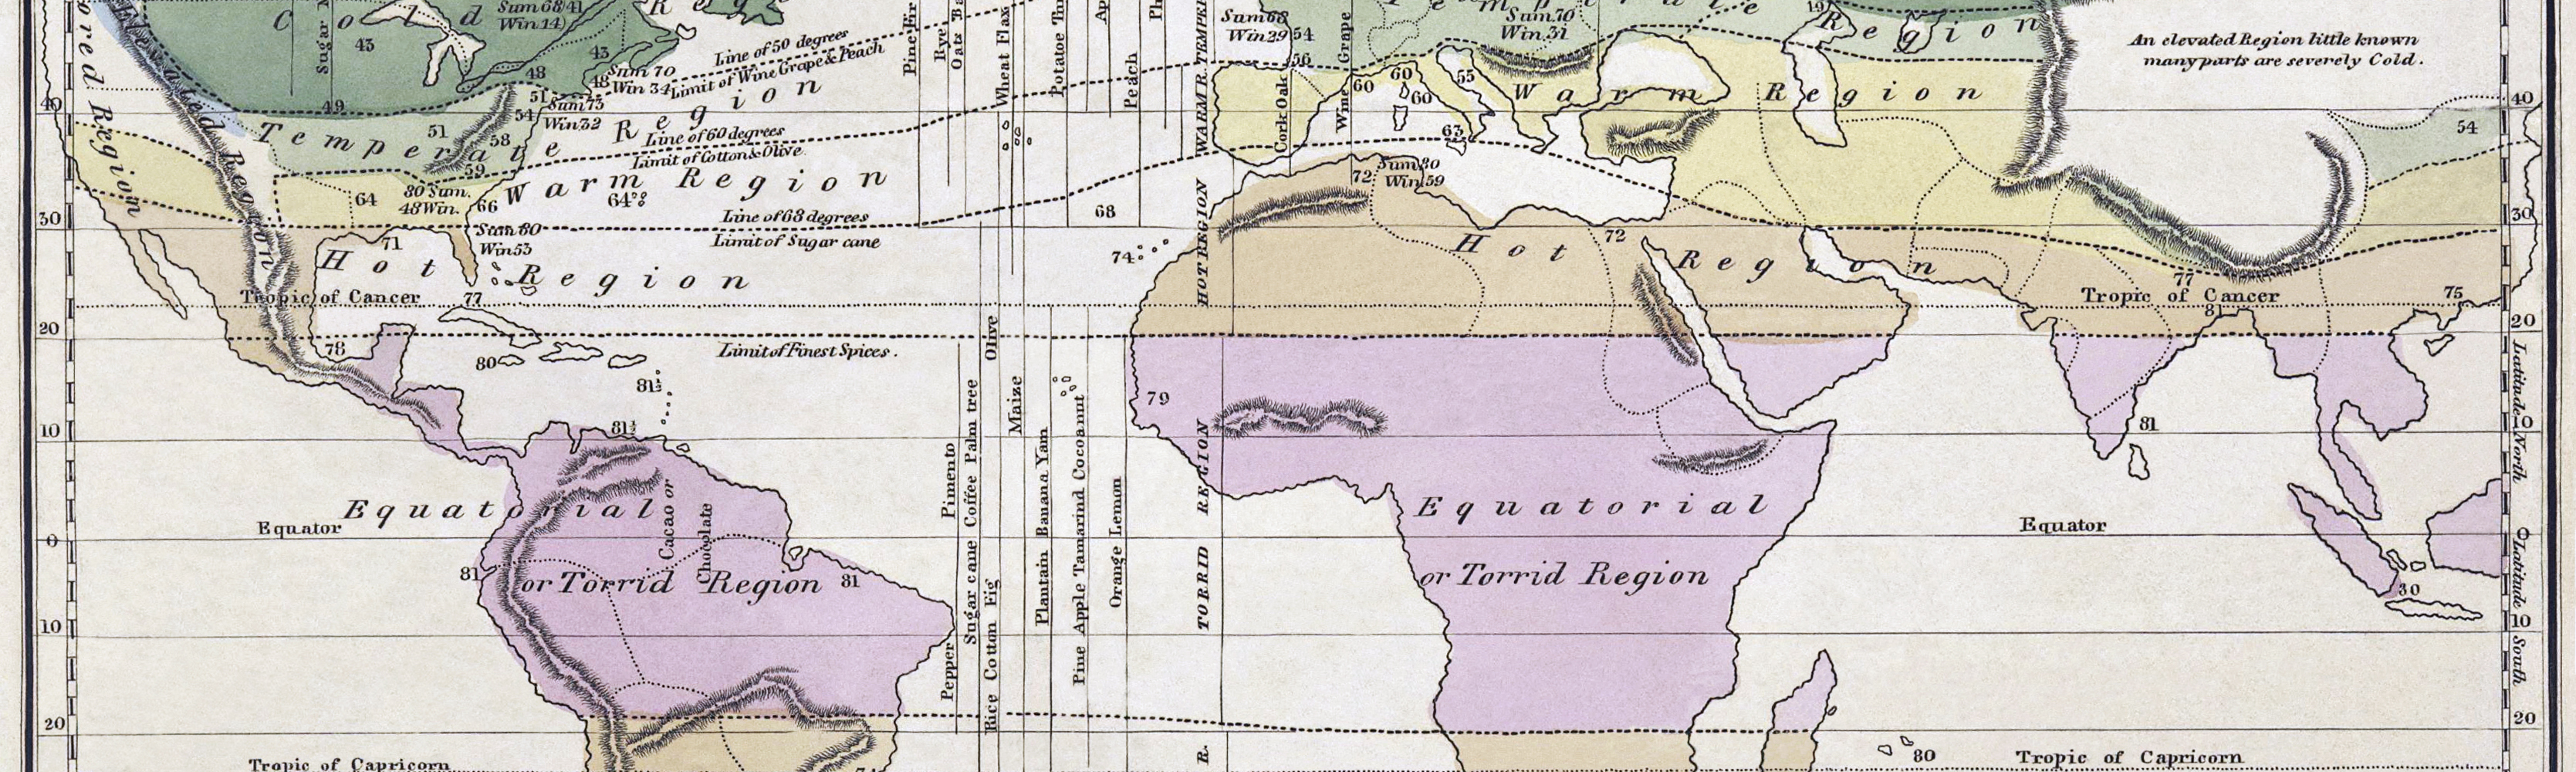
\includegraphics[width=.9\linewidth,height=.225\paperheight]{../../pictures/Woodbridge_isothermal_chart3-2.jpg}}
        \caption{\footnotesize W.C. Woodbridge, \emph{Isothermal Chart} (1823). Public domain.}
    \end{centering}
    %\end{adjustwidth}
\end{figure}

\lettrine[lines=4]{\goudy T}{he} periodic changes of temperature which have been occasioned on the Earth's surface by the Sun's position and by meteorological processes are continued in its interior, although to a very inconsiderable depth. The slow conducting power of the ground diminishes this loss of heat in the winter and is very favorable to deep-rooted trees. Points that lie at very different depths on the same vertical line attain the maximum and minimum of the imparted temperature at very different periods of time. The further they are removed from the surface, the smaller is this difference between the extremes. In the latitudes of our temperate zone (between 48 and 52), the stratum of invariable temperature is at a depth of from 59 to 64 feet, and at half that depth the oscillations of the thermometer, from the influence of the seasons, scarcely amount to half a degree. In tropical climates, this invariable stratum is only one foot below the surface, and this fact has been ingeniously made use of by Boussingault to obtain a convenient, and, as he believes, certain determination of the mean temperature of the air of different places. This mean temperature of the air at a fixed point, or at a group of contiguous points on the surface, is to a certain degree the fundamental element of the climate and agricultural relations of a district; but the mean temperature of the whole surface is very different from that of the globe itself. The questions so often agitated, whether the mean temperature has experienced any considerable differences in the course of centuries, whether the climate of a country has deteriorated, and whether the winters have not become milder and the summers cooler, can only be answered by means of the thermometer; this instrument has, however, scarcely been invented more than two centuries and a half, and its scientific application hardly dates back 120 years. The nature and novelty of the means interpose, therefore, very narrow limits to our investigation regarding the temperature of the air. It is quite otherwise, however, with the solution of the great problem of the internal heat of the whole Earth. As we may judge of uniformity of temperature from the unaltered time of vibration of a pendulum, so we may also learn, from the unaltered rotatory velocity of the Earth, the amount of stability in the mean temperature of our globe. This insight into the relations between the length of the day and the heat of the Earth is the result of one of the most brilliant applications of the knowledge we had long possessed of the movement of the heavens to the thermic condition of our planet. The rotatory velocity of the Earth depends on its volume; and since, by the gradual cooling of the mass by radiation, the axis of rotation would become shorter, the rotatory velocity would necessarily increase, and the length of the day diminish, with a decrease of the temperature. From the comparison of the secular inequalities in the motions of the Moon with the eclipses observed in ancient times, it follows that, since the time of Hipparchus, that is, for full 2000 years, the length of the day has certainly not diminished by the hundredth part of a second. The decrease of the mean heat of the globe during a period of 2000 years has not, therefore, taking the extremest limits, diminished as much as 535th of a degree of Fahrenheit.\footnote{Laplace, Exp. du Syst. du Monde, p. 229 and 263; M\'{e}caniqueC\'{e}leste, t. v., p. 18 and 72, It should be remarked that the fractionsooth of a degree of Fahrenheit of the mercurial thermometer, given inthe text as the limit of the stability of the Earths temperature sincthe days of Hipparchus, rests on the assumption that the dilatation ofthe substances of which the Earth is composed is equal to that of glass, that is to say, g.hyath for 1. Regarding this hypathsis, see Aragain the Annuaire for 1834, p. 177190.}

This invariability of form presupposes also a great invariability in the distribution of relations of density in the interiorof the globe. The translatory movements, which occasionthe eruptions of our present volcanoes and of ferruginous lava,and the filling up of previously empty fissures and cavitieswith dense masses of stone, are consequently only to be regarded as slight superficial phenomena aflecting merely oneportion of the Earths crust, which, from their smallnesswhen compared to the Karths radius, become wholly insignificant.